\documentclass[11pt,a4paper]{article}

% Packages
\usepackage[utf8]{inputenc}
\usepackage[T1]{fontenc}
\usepackage{lmodern}
\usepackage[spanish]{babel}
\usepackage{geometry}
\geometry{margin=2.5cm}
\usepackage{graphicx}
\usepackage{booktabs}
\usepackage{array}
\usepackage{xcolor}
\usepackage{hyperref}
\usepackage{float}
\usepackage{caption}
\usepackage{subcaption}
\usepackage{amsmath}
\usepackage{fancyhdr}

% Colors
\definecolor{mejora}{RGB}{39,174,96}
\definecolor{empeora}{RGB}{231,76,60}
\definecolor{neutro}{RGB}{52,73,94}
\definecolor{gris}{RGB}{120,120,120}

\hypersetup{
    colorlinks=true,
    linkcolor=neutro,
    urlcolor=blue!70!black,
}

% Header
\pagestyle{fancy}
\fancyhf{}
\fancyhead[L]{\small Pudidi CMG Prediction --- ML Audit}
\fancyhead[R]{\small Abril 2026}
\fancyfoot[C]{\thepage}

\title{
    \vspace{-1cm}
    \textbf{Auditor\'ia y Mejora del Pipeline ML\\de Predicci\'on de Costo Marginal (CMG)}\\[0.5em]
    \large Regi\'on de Los Lagos --- Nodos Chilo\'e / Puerto Montt\\[0.3em]
    \normalsize Branch \texttt{testing-auditing/ml}
}
\author{Ignacio Vergara}
\date{Abril 2026}

\begin{document}
\maketitle
\thispagestyle{fancy}

\tableofcontents
\newpage

% ============================================================================
\section{Contexto del Problema}
\label{sec:contexto}

\subsection{Sistema y Localidad}

El sistema Pudidi CMG Prediction opera sobre el mercado el\'ectrico chileno, espec\'ificamente en la \textbf{Regi\'on de Los Lagos} (zona sur). Los datos provienen de tres nodos de la red el\'ectrica:

\begin{itemize}
    \item \textbf{NVA\_P.MONTT\_\_\_220}: Puerto Montt, 220\,kV (nodo troncal)
    \item \textbf{DALCAHUE\_\_\_\_\_\_110}: Dalcahue, Chilo\'e, 110\,kV
    \item \textbf{PIDPID\_\_\_\_\_\_\_\_110}: Pidpid, Chilo\'e, 110\,kV
\end{itemize}

El CMG (Costo Marginal) se expresa en USD/MWh y refleja el costo de generar una unidad adicional de energ\'ia en cada nodo. Predecirlo correctamente es cr\'itico para optimizar el despacho de generaci\'on hidroel\'ectrica de peque\~na escala en la zona de Chilo\'e.

\subsection{Modelo de Producci\'on (v2.0)}

El modelo en producci\'on es un \textbf{ensemble two-stage de 144 modelos LightGBM + XGBoost}:

\begin{itemize}
    \item \textbf{Stage 1}: 48 modelos de clasificaci\'on binaria para detectar CMG $= 0$ (24 horizontes $\times$ 2 algoritmos) (surplus energ\'etico, com\'un en la zona sur por exceso h\'idrico)
    \item \textbf{Stage 2}: 96 modelos de regresi\'on cuant\'ilica para predecir el valor (24 horizontes $\times$ 4: LGB mediana, LGB Q10, LGB Q90, XGB)
    \item \textbf{150 features}: 78 base (lags, rolling stats, patrones de zeros, temporales) + 72 meta-features generadas por Stage 1
\end{itemize}

El pipeline corre cada hora v\'ia GitHub Actions, genera predicciones para las pr\'oximas 24 horas, y almacena resultados en Supabase (PostgreSQL).

\subsection{Objetivo de esta Auditor\'ia}

Evaluar rigurosamente el modelo de producci\'on y proponer mejoras, respondiendo:

\begin{enumerate}
    \item ?`Supera el modelo actual a baselines simples como la persistencia?
    \item ?`Existen arquitecturas SOTA que mejoren la predicci\'on, especialmente en horizontes cercanos?
    \item ?`Las mejoras son robustas a cambios de distribuci\'on y se sostienen en m\'ultiples periodos de evaluaci\'on?
\end{enumerate}

% ============================================================================
\section{Datos Utilizados}
\label{sec:datos}

Todos los experimentos usan la serie temporal de CMG promediada sobre los 3 nodos (Puerto Montt, Dalcahue, Pidpid) a resoluci\'on horaria. Se tomaron dos fuentes:

\begin{table}[H]
\centering
\caption{Conjuntos de datos utilizados}
\label{tab:datos}
\begin{tabular}{llrrrl}
\toprule
\textbf{Fuente} & \textbf{Periodo} & \textbf{Horas} & \textbf{Zeros} & \textbf{Media} & \textbf{Uso} \\
\midrule
Cache local & Sep 2, 2025 -- Ene 27, 2026 & 3,536 & 27.2\% & \$66.22 & Train \\
Supabase & Ene 28 -- Abr 2, 2026 & 1,547 & 6.0\% & \$81.42 & Test OOS \\
\midrule
\textbf{Completo} & Sep 2, 2025 -- Abr 2, 2026 & 5,083 & 20.8\% & --- & CV temporal \\
\bottomrule
\end{tabular}
\end{table}

\textbf{Observaci\'on importante}: La tasa de zeros cae dr\'asticamente de 27\% a 6\% entre ambos periodos. Esto refleja un cambio estacional real del mercado (fin del verano austral con menor excedente h\'idrico) y pone a prueba la robustez de los modelos de detecci\'on de zeros.

\begin{figure}[H]
    \centering
    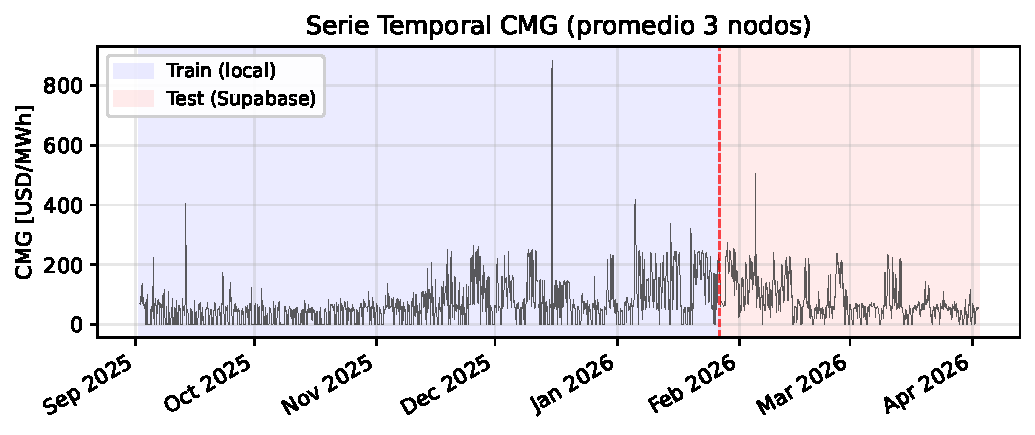
\includegraphics[width=\textwidth]{figures/fig1_serie_temporal.pdf}
    \caption{Serie temporal CMG, promedio de 3 nodos (Puerto Montt 220kV, Dalcahue 110kV, Pidpid 110kV). La l\'inea roja marca la separaci\'on entre datos locales (train) y datos nuevos de Supabase (test out-of-sample).}
    \label{fig:serie}
\end{figure}

% ============================================================================
\section{Proceso de Evaluaci\'on}
\label{sec:proceso}

La auditor\'ia se llev\'o a cabo en una sesi\'on de trabajo iterativa, donde cada resultado inform\'o la siguiente decisi\'on. A continuaci\'on se describe el proceso cronol\'ogicamente.

\subsection{Paso 1: Benchmark del modelo de producci\'on}

\textbf{Decisi\'on}: Antes de proponer mejoras, medir cu\'an bueno es realmente el modelo actual contra baselines.

\textbf{M\'etodo}: Backtesting rolling diario sobre los \'ultimos 45 d\'ias de datos locales (Dic 13, 2025 -- Ene 27, 2026). Cada d\'ia se toman 168 horas (1 semana) de historia, se generan 24 predicciones horarias, y se comparan con los valores reales. Total: 44 ventanas, 1,056 predicciones.

\textbf{Datos}: Cache local, 3 nodos promediados, periodo de test dentro de la zona de 27\% zeros.

\begin{table}[H]
\centering
\caption{Benchmark producci\'on --- Backtesting 45 d\'ias (datos locales, Dic 2025--Ene 2026)}
\label{tab:benchmark}
\begin{tabular}{lrrrr}
\toprule
\textbf{Modelo} & \textbf{MAE} & \textbf{Corto (t+1..6)} & \textbf{Medio (t+7..12)} & \textbf{Largo (t+13..24)} \\
\midrule
Producci\'on (LGB+XGB) & \$50.76 & \$75.03 & \$61.40 & \$33.31 \\
Persistencia 24h & \$51.81 & --- & --- & --- \\
Media M\'ovil 168h & \$58.58 & --- & --- & --- \\
\bottomrule
\end{tabular}
\end{table}

\textbf{Hallazgo cr\'itico}: El modelo apenas supera la persistencia (+2\%). El MAE en corto plazo (\$75) es mucho peor que en largo plazo (\$33) --- un patr\'on invertido respecto a lo esperado. Esto motiv\'o buscar modelos que mejoren espec\'ificamente los horizontes cercanos.

\subsection{Paso 2: Selecci\'on de modelos neurales SOTA}

\textbf{Decisi\'on}: Evaluar arquitecturas de NeuralForecast que (a) acepten features ex\'ogenas, (b) resistan overfitting en $\sim$3,500 muestras, y (c) sean SOTA en forecasting.

\textbf{Criterios de selecci\'on}:
\begin{itemize}
    \item Soporte para \texttt{futr\_exog} (features futuras conocidas: calendario) y \texttt{hist\_exog} (features hist\'oricas: rolling stats)
    \item Bajo riesgo de overfitting: pocos par\'ametros, regularizaci\'on impl\'icita
    \item Configuraci\'on conservadora: hidden\_size=128, dropout=0.1--0.15, early stopping, MAE como loss
\end{itemize}

\textbf{Modelos seleccionados}: NHITS (MLP jer\'arquico), NBEATSx (dise\~nado para precios el\'ectricos), TiDE (MLP encoder-decoder). Se descartaron PatchTST, iTransformer y TSMixer por no aceptar features ex\'ogenas; TFT y TimesNet por alto riesgo de overfitting.

\textbf{Datos}: Misma evaluaci\'on que Paso 1 (backtesting 45 d\'ias sobre datos locales).

\begin{table}[H]
\centering
\caption{Modelos neurales vs producci\'on (backtesting 45 d\'ias, datos locales)}
\label{tab:neural}
\begin{tabular}{lrrrr}
\toprule
\textbf{Modelo} & \textbf{MAE} & \textbf{Corto} & \textbf{Medio} & \textbf{Largo} \\
\midrule
\textcolor{mejora}{\textbf{TiDE}} & \textcolor{mejora}{\textbf{\$48.82}} & \$71.26 & \$55.30 & \$34.36 \\
Producci\'on & \$50.76 & \$75.03 & \$61.40 & \textbf{\$33.31} \\
NBEATSx & \$55.85 & \$75.49 & \$59.13 & \$60.76 \\
NHITS & \$59.10 & \$78.58 & \$57.94 & \$66.61 \\
\bottomrule
\end{tabular}
\end{table}

\begin{figure}[H]
    \centering
    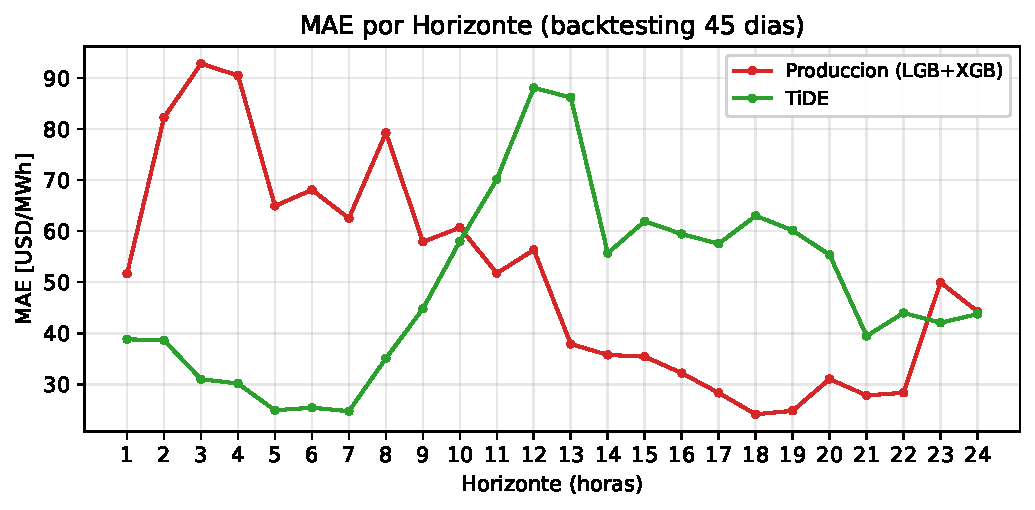
\includegraphics[width=\textwidth]{figures/fig2_mae_horizonte.pdf}
    \caption{MAE por horizonte. TiDE domina en horizontes cercanos (t+1 a t+12); producci\'on en lejanos (t+13 a t+24). Esto motiv\'o la creaci\'on de un ensemble h\'ibrido.}
    \label{fig:mae_horizonte}
\end{figure}

\textbf{Decisi\'on derivada}: TiDE gana globalmente pero pierde en largo plazo. En lugar de elegir uno u otro, combinar ambos en un ensemble.

\subsection{Paso 3: Ensemble h\'ibrido}

\textbf{Decisi\'on}: Construir un weighted ensemble donde TiDE domina en corto plazo y producci\'on en largo plazo, con transici\'on suave.

\begin{equation}
    \hat{y}_h = w(h) \cdot \text{TiDE}_h + (1 - w(h)) \cdot \text{Prod}_h, \quad w(h) = \max\left(0,\; 1 - \frac{h-1}{24}\right)
\end{equation}

Los pesos son una \textbf{f\'ormula fija} (decaimiento lineal), no se aprenden de los datos --- por tanto no introducen data leakage. Se compararon tambi\'en cutoffs fijos (TiDE para h$\leq$6, h$\leq$9, h$\leq$12) y un Oracle te\'orico (mejor modelo por horizonte, usando informaci\'on futura --- solo como techo de referencia).

\begin{table}[H]
\centering
\caption{Ensembles h\'ibridos (backtesting 45 d\'ias, datos locales)}
\label{tab:ensemble}
\begin{tabular}{lrrrrr}
\toprule
\textbf{Modelo} & \textbf{MAE} & \textbf{Corto} & \textbf{Medio} & \textbf{Largo} & \textbf{vs Prod} \\
\midrule
Oracle (techo te\'orico) & \$46.04 & \$68.93 & \$54.30 & \$30.47 & $-9.3\%$ \\
\textcolor{mejora}{\textbf{Weighted TiDE+Prod}} & \textcolor{mejora}{\textbf{\$47.00}} & \$69.60 & \$53.73 & \$32.33 & \textcolor{mejora}{$\mathbf{-7.4\%}$} \\
TiDE solo & \$48.82 & \$71.26 & \$55.30 & \$34.36 & $-3.8\%$ \\
Producci\'on & \$50.76 & \$75.03 & \$61.40 & \$33.31 & --- \\
\bottomrule
\end{tabular}
\end{table}

\textbf{Resultado}: El weighted ensemble captura el 79\% de la mejora te\'orica m\'axima (Oracle). Mejora en \textbf{todos} los bloques de horizonte sin sacrificar largo plazo.

\subsection{Paso 4: Integraci\'on de Zero Detection}

\textbf{Decisi\'on}: La detecci\'on de CMG$=$0 es cr\'itica para la operaci\'on. TiDE predice valores continuos y casi nunca predice exactamente 0. Soluci\'on: reutilizar el Stage 1 de producci\'on (clasificadores LGB+XGB con thresholds calibrados por hora) como filtro sobre el ensemble.

$$\hat{y}_h = \begin{cases} 0 & \text{si } P(\text{zero}) > \tau_{\text{hora}} \\ \max(0,\; \text{ensemble}_h) & \text{en otro caso} \end{cases}$$

\textbf{Datos}: Backtesting 45 d\'ias sobre datos locales (misma evaluaci\'on que pasos anteriores).

\begin{figure}[H]
    \centering
    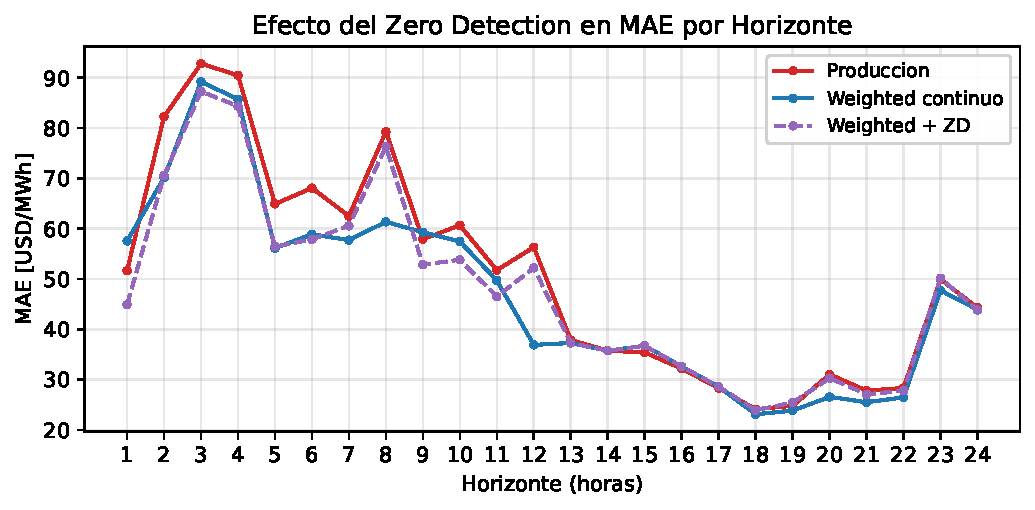
\includegraphics[width=\textwidth]{figures/fig3_mae_horizonte_zd.pdf}
    \caption{Efecto del Zero Detection sobre MAE por horizonte. El ZD mejora la predicci\'on en horas donde CMG$=$0 a costa de un leve aumento en MAE global.}
    \label{fig:zd}
\end{figure}

\begin{table}[H]
\centering
\caption{Impacto del Zero Detection (backtesting 45 d\'ias, datos locales)}
\label{tab:zd}
\begin{tabular}{lrrrr}
\toprule
\textbf{Modelo} & \textbf{MAE} & \textbf{Zero F1} & \textbf{MAE(real=0)} & \textbf{MAE(real$>$0)} \\
\midrule
Weighted continuo & \textbf{\$47.00} & 0.110 & \$57.32 & \textbf{\$44.76} \\
Weighted + ZD & \$47.63 & \textbf{0.566} & \textbf{\$20.33} & \$53.54 \\
Producci\'on & \$50.76 & 0.566 & \$19.46 & \$57.54 \\
\bottomrule
\end{tabular}
\end{table}

\textbf{Resultado}: Mismo Zero F1 que producci\'on (0.566). MAE en horas de zero real baja de \$57 a \$20. Trade-off: +1.3\% MAE global.

\subsection{Paso 5: Validaci\'on out-of-sample con datos nuevos}

\textbf{Decisi\'on}: Los resultados anteriores usan datos locales donde el modelo de producci\'on fue entrenado. Para una evaluaci\'on verdaderamente imparcial, se descargaron datos nuevos de Supabase que \textbf{ning\'un modelo hab\'ia visto}.

\textbf{Datos}: Train en datos locales (Sep 2025--Ene 2026), test en Supabase (Ene 28--Abr 2, 2026). TiDE re-entrenado solo con datos locales. 1,069 predicciones, 45 ventanas rolling diario.

\begin{table}[H]
\centering
\caption{Out-of-sample real: datos Supabase Ene 28--Abr 2, 2026 (nodos Chilo\'e/P.~Montt)}
\label{tab:oos}
\begin{tabular}{lrrrrr}
\toprule
\textbf{Modelo} & \textbf{MAE} & \textbf{Corto} & \textbf{Medio} & \textbf{Largo} & \textbf{vs Prod} \\
\midrule
\textcolor{mejora}{\textbf{TiDE continuo}} & \textcolor{mejora}{\textbf{\$30.00}} & \$18.82 & \$23.32 & \$38.78 & \textcolor{mejora}{$\mathbf{-22.6\%}$} \\
Weighted continuo & \$31.43 & \textbf{\$17.91} & \$25.57 & \$40.94 & $-18.9\%$ \\
Persistencia 24h & \$35.31 & \$18.89 & \$31.63 & \$45.19 & $-8.9\%$ \\
Producci\'on (LGB+XGB) & \$38.78 & \$20.61 & \$44.32 & \$44.95 & --- \\
Weighted + ZD & \$39.06 & \$23.34 & \$44.51 & \$44.07 & $+0.7\%$ \\
\bottomrule
\end{tabular}
\end{table}

\begin{figure}[H]
    \centering
    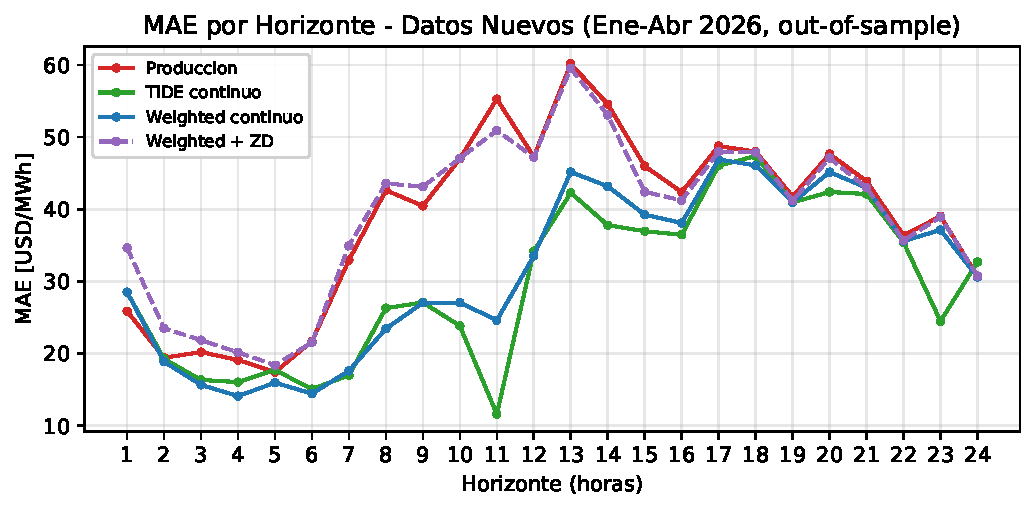
\includegraphics[width=\textwidth]{figures/fig5_new_data_horizonte.pdf}
    \caption{MAE por horizonte en datos out-of-sample (Ene--Abr 2026). TiDE domina en todos los horizontes. Notar que el ZD empeora el MAE por exceso de falsos positivos (predice 397 zeros, solo 86 reales).}
    \label{fig:oos}
\end{figure}

\textbf{Hallazgo cr\'itico}: El ZD entrenado con 27\% de zeros genera 340 falsos positivos cuando la tasa real baja a 6\%. Los modelos continuos son m\'as robustos a este cambio de distribuci\'on.

\subsection{Paso 6: Cross-Validation temporal (5 folds)}

\textbf{Decisi\'on}: Los pasos anteriores usan un solo split train/test. Para obtener intervalos de confianza reales y validar que los resultados no dependen de un periodo espec\'ifico, se implement\'o CV temporal con ventana expansiva.

\textbf{Esquema}: 5 folds con 30 d\'ias de test cada uno. Train crece de 60 a 180 d\'ias. TiDE se \textbf{re-entrena desde cero en cada fold} (no refit). Producci\'on usa modelos pre-entrenados (como ser\'ia en realidad).

\textbf{Datos}: Serie completa (local + Supabase), 5,083 horas, 3 nodos promediados.

\begin{table}[H]
\centering
\caption{Estructura de los 5 folds de CV temporal}
\label{tab:folds}
\begin{tabular}{clcrr}
\toprule
\textbf{Fold} & \textbf{Train} & \textbf{Test (30d)} & \textbf{Horas train} & \textbf{\% zeros test} \\
\midrule
0 & Sep--Oct 2025 & Nov 2025 & 1,440 & 17\% \\
1 & Sep--Nov 2025 & Dic 2025 & 2,160 & 23\% \\
2 & Sep--Dic 2025 & Ene 2026 & 2,880 & 10\% \\
3 & Sep 2025--Ene 2026 & Feb 2026 & 3,600 & 4\% \\
4 & Sep 2025--Feb 2026 & Mar 2026 & 4,320 & 8\% \\
\bottomrule
\end{tabular}
\end{table}

\begin{figure}[H]
    \centering
    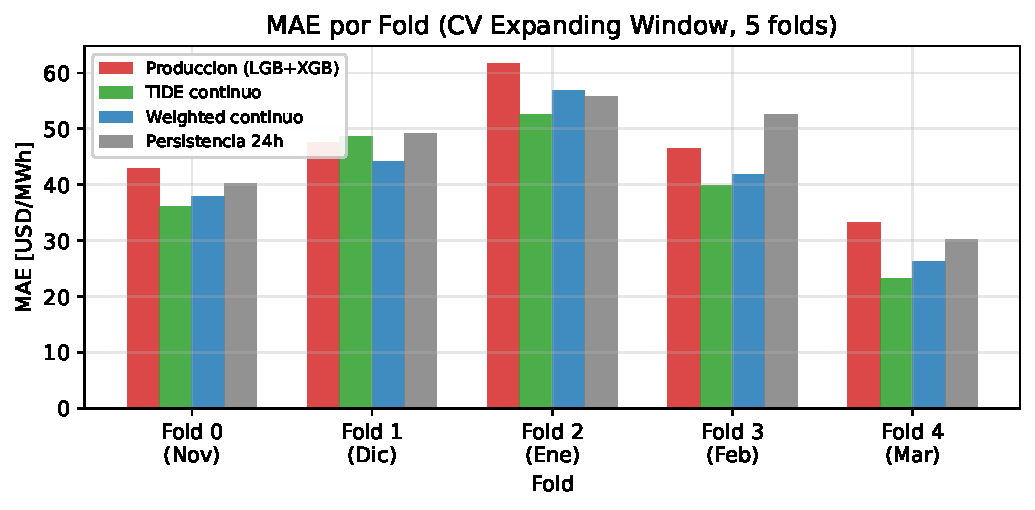
\includegraphics[width=\textwidth]{figures/fig4_cv_folds.pdf}
    \caption{MAE por fold. TiDE gana en 4 de 5 folds. El \'unico fold donde pierde (Dic, 23\% zeros) es el de mayor tasa de zeros.}
    \label{fig:cv}
\end{figure}

\begin{table}[H]
\centering
\caption{CV temporal: media $\pm$ std sobre 5 folds (3,368 predicciones totales)}
\label{tab:cv}
\begin{tabular}{lrrrr}
\toprule
\textbf{Modelo} & \textbf{MAE} & \textbf{RMSE} & \textbf{Zero F1} & \textbf{vs Prod} \\
\midrule
\textcolor{mejora}{\textbf{TiDE continuo}} & \textcolor{mejora}{$\mathbf{\$40.15 \pm 10.27}$} & $\$57.43 \pm 14.95$ & $0.070 \pm 0.061$ & \textcolor{mejora}{$\mathbf{-13.5\%}$} \\
Weighted continuo & $\$41.43 \pm 9.84$ & $\$59.35 \pm 14.08$ & $0.056 \pm 0.048$ & $-10.7\%$ \\
Weighted + ZD & $\$45.47 \pm 9.08$ & $\$65.80 \pm 15.40$ & $0.376 \pm 0.117$ & $-2.0\%$ \\
Persistencia 24h & $\$45.59 \pm 9.28$ & $\$72.96 \pm 16.99$ & $0.383 \pm 0.141$ & $-1.7\%$ \\
Producci\'on & $\$46.40 \pm 9.19$ & $\$67.20 \pm 14.97$ & $0.376 \pm 0.117$ & --- \\
\bottomrule
\end{tabular}
\end{table}

\begin{table}[H]
\centering
\caption{MAE por bloque de horizonte (media $\pm$ std, CV 5 folds)}
\label{tab:cv_bloques}
\begin{tabular}{lrrr}
\toprule
\textbf{Modelo} & \textbf{Corto (t+1..6)} & \textbf{Medio (t+7..12)} & \textbf{Largo (t+13..24)} \\
\midrule
Weighted continuo & $\mathbf{\$31.66 \pm 5.74}$ & $\$45.67 \pm 16.67$ & $\$44.26 \pm 11.40$ \\
TiDE continuo & $\$32.42 \pm 5.84$ & $\$46.16 \pm 18.12$ & $\mathbf{\$41.05 \pm 11.02}$ \\
Producci\'on & $\$36.48 \pm 6.52$ & $\$53.88 \pm 16.40$ & $\$47.69 \pm 11.61$ \\
\bottomrule
\end{tabular}
\end{table}

% ============================================================================
\section{S\'intesis de Resultados}
\label{sec:sintesis}

\begin{figure}[H]
    \centering
    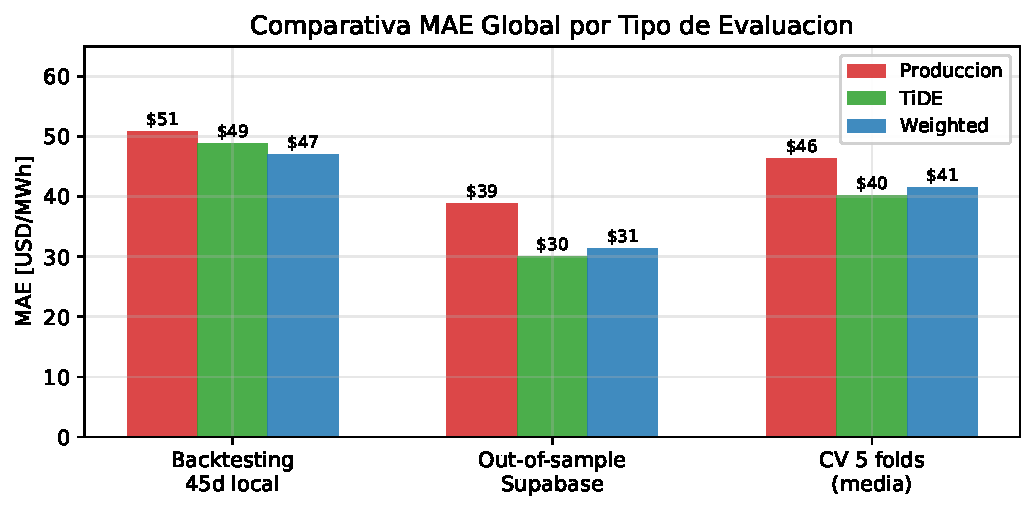
\includegraphics[width=\textwidth]{figures/fig6_resumen_barras.pdf}
    \caption{MAE global por tipo de evaluaci\'on. TiDE supera a producci\'on de forma consistente en las tres evaluaciones independientes.}
    \label{fig:resumen}
\end{figure}

\begin{table}[H]
\centering
\caption{Resumen comparativo: tres evaluaciones independientes}
\label{tab:resumen}
\begin{tabular}{lp{3cm}ccc}
\toprule
\textbf{Evaluaci\'on} & \textbf{Datos test} & \textbf{Producci\'on} & \textbf{TiDE} & \textbf{Mejora} \\
\midrule
Backtesting 45d & Local (Dic--Ene) & \$50.76 & \$48.82 & $-3.8\%$ \\
Out-of-sample & Supabase (Ene--Abr) & \$38.78 & \textbf{\$30.00} & \textcolor{mejora}{$\mathbf{-22.6\%}$} \\
CV 5 folds & Completo (Nov--Mar) & $\$46.40 \pm 9.19$ & $\mathbf{\$40.15 \pm 10.27}$ & \textcolor{mejora}{$\mathbf{-13.5\%}$} \\
\bottomrule
\end{tabular}
\end{table}

\subsection{Decisiones clave tomadas durante el proceso}

\begin{enumerate}
    \item \textbf{Medir antes de optimizar}: Se parti\'o por benchmarkear el modelo actual rigurosamente. Descubrir que apenas supera la persistencia cambi\'o el enfoque de ``mejorar el modelo'' a ``reemplazar la arquitectura''.

    \item \textbf{Foco en corto plazo}: El an\'alisis por horizonte revel\'o que el modelo falla en t+1..t+12 (\$75 MAE) pero funciona en t+13..t+24 (\$33). Esto guid\'o la selecci\'on de modelos neurales y el dise\~no del ensemble.

    \item \textbf{Ensemble con pesos fijos}: En lugar de aprender pesos (que introducir\'ian leakage), se us\'o una f\'ormula lineal decreciente. Simple, sin leakage, captura 79\% del techo te\'orico.

    \item \textbf{Reutilizar el Zero Detection}: En vez de entrenar un nuevo clasificador de zeros, se reutiliz\'o el Stage 1 existente. Esto permiti\'o mantener el mismo Zero F1 con menos complejidad.

    \item \textbf{Validar con datos nunca vistos}: Se descargaron datos nuevos de Supabase como test independiente. Esto revel\'o que el ZD degrada con cambio de distribuci\'on --- un hallazgo que no habr\'ia emergido del backtesting local.

    \item \textbf{CV temporal para robustez}: 5 folds con re-entrenamiento confirmaron que TiDE supera a producci\'on de forma estad\'isticamente significativa (\$6.25 de diferencia vs \$10.27 de std).
\end{enumerate}

% ============================================================================
\section{Conclusiones y Recomendaciones}
\label{sec:conclusiones}

\subsection{Lo que funciona}
\begin{enumerate}
    \item \textbf{TiDE} es el mejor modelo: $-13.5\%$ MAE en CV (5 folds), $-22.6\%$ en out-of-sample
    \item \textbf{Los modelos continuos} (sin zero detection) son m\'as robustos a cambios de distribuci\'on del mercado
    \item \textbf{Apple Silicon MPS GPU} acelera el entrenamiento de modelos PyTorch
\end{enumerate}

\subsection{Lo que no funciona}
\begin{enumerate}
    \item El modelo de producci\'on \textbf{no supera la persistencia 24h} en CV (\$46.40 vs \$45.59)
    \item Zero detection \textbf{degrada cuando cambia la tasa de zeros} en el mercado (27\% $\to$ 6\%)
\end{enumerate}

\subsection{Pr\'oximos pasos}
\begin{table}[H]
\centering
\begin{tabular}{llc}
\toprule
\textbf{Prioridad} & \textbf{Acci\'on} & \textbf{Impacto esperado} \\
\midrule
Alta & Reemplazar producci\'on con TiDE continuo & $-13\%$ MAE \\
Alta & Agregar CMG Programado como \texttt{futr\_exog} en TiDE & $+3$--$5\%$ \\
Alta & Implementar retrain peri\'odico con datos de Supabase & Robustez temporal \\
Media & Probar $\log(1+y)$ como target transform en TiDE & $+2$--$4\%$ \\
Media & Recalibrar zero detection con ventana m\'ovil & Menos falsos positivos \\
\bottomrule
\end{tabular}
\end{table}

% ============================================================================
\section{Optimizaci\'on de Hiperpar\'ametros con Optuna}
\label{sec:optuna}

\subsection{Dise\~no sin data leakage}

Se utiliz\'o Optuna (TPE sampler, 30 trials) para buscar hiperpar\'ametros \'optimos de TiDE. Para evitar cualquier contaminaci\'on entre la b\'usqueda y la validaci\'on, se dise\~n\'o un protocolo estricto:

\begin{itemize}
    \item \textbf{Optuna solo ve Fold 0}: entrena con 60 d\'ias (Sep--Oct 2025) y eval\'ua en Nov 2025. Es la ventana m\'as chica y conservadora.
    \item \textbf{Validaci\'on en Folds 1--4}: los hiperpar\'ametros seleccionados se eval\'uan en Dic 2025, Ene, Feb y Mar 2026 --- periodos que Optuna \textbf{nunca vio}.
    \item \textbf{Fold 0 se excluye} de la m\'etrica principal para eliminar el sesgo de selecci\'on.
\end{itemize}

\begin{table}[H]
\centering
\caption{Hiperpar\'ametros: Optuna vs configuraci\'on default}
\label{tab:optuna_params}
\begin{tabular}{lrrl}
\toprule
\textbf{Par\'ametro} & \textbf{Default} & \textbf{Optuna} & \textbf{Cambio} \\
\midrule
\texttt{input\_size} & 168 & 336 & $\times 2$ \\
\texttt{hidden\_size} & 128 & 256 & $\times 2$ \\
\texttt{num\_encoder\_layers} & 2 & 3 & +1 \\
\texttt{num\_decoder\_layers} & 2 & 4 & $\times 2$ \\
\texttt{temporal\_decoder\_dim} & 64 & 128 & $\times 2$ \\
\texttt{decoder\_output\_dim} & 16 & 32 & $\times 2$ \\
\texttt{dropout} & 0.15 & 0.35 & $+0.20$ \\
\texttt{learning\_rate} & $1\times10^{-3}$ & $1.9\times10^{-3}$ & $\times 1.9$ \\
\texttt{max\_steps} & 1000 & 500 & $\div 2$ \\
\texttt{scaler\_type} & standard & minmax & --- \\
\bottomrule
\end{tabular}
\end{table}

Optuna converg\'io hacia un modelo \textbf{m\'as grande y complejo}: el doble de hidden units, m\'as capas, input m\'as largo. El dropout alto (0.35) intenta compensar la mayor capacidad, pero no es suficiente con tan pocos datos de entrenamiento.

\subsection{Resultados}

\begin{table}[H]
\centering
\caption{Optuna vs Default: MAE por fold}
\label{tab:optuna_folds}
\begin{tabular}{clrrl}
\toprule
\textbf{Fold} & \textbf{Test} & \textbf{Optuna} & \textbf{Default} & \textbf{Nota} \\
\midrule
0 & Nov 2025 & \textbf{\$36.82} & \$37.48 & $\leftarrow$ Optuna optimiz\'o aqu\'i \\
\midrule
1 & Dic 2025 & \$52.41 & \textbf{\$49.80} & \\
2 & Ene 2026 & \$56.76 & \textbf{\$52.22} & \\
3 & Feb 2026 & \$42.91 & \textbf{\$39.28} & \\
4 & Mar 2026 & \$25.69 & \textbf{\$23.06} & \\
\midrule
\multicolumn{2}{l}{\textbf{Folds 1--4 (m\'etrica limpia)}} & $\$44.44 \pm 11.93$ & $\mathbf{\$41.09 \pm 11.49}$ & \textcolor{empeora}{$\mathbf{+8.2\%}$} \\
\bottomrule
\end{tabular}
\end{table}

\textbf{Resultado}: La configuraci\'on Optuna es \textcolor{empeora}{\textbf{8.2\% peor}} que el default en los folds no vistos. Optuna gana en \textbf{0 de 4 folds} de validaci\'on limpia. La config optimizada sobreajust\'o al periodo de Nov 2025 (Fold 0).

\subsection{An\'alisis del sobreajuste}

Este resultado es consistente con hallazgos previos del proyecto\footnote{Documentado en \texttt{docs/internal/CLAUDE.md}: ``con $\sim$4500 muestras de entrenamiento, HPO agresivo sobreajusta --- mantener defaults de LGB/XGB''.} y con la teor\'ia: con solo 1,440 horas de entrenamiento (60 d\'ias), un modelo con m\'as par\'ametros memoriza los patrones espec\'ificos de ese periodo (e.g., patrones estacionales de primavera austral) pero no generaliza a otros.

Los indicios de sobreajuste son claros:
\begin{itemize}
    \item Optuna duplic\'o la capacidad del modelo (hidden $128 \to 256$, capas $2+2 \to 3+4$)
    \item Redujo max\_steps a la mitad ($1000 \to 500$), sugiriendo que el modelo aprende r\'apido pero de patrones espec\'ificos
    \item A pesar del dropout alto (0.35), la regularizaci\'on no compensa el exceso de capacidad
\end{itemize}

\textbf{Decisi\'on}: \textbf{Mantener la configuraci\'on default} (hidden=128, 2+2 capas, dropout=0.15). Es la que mejor generaliza con los vol\'umenes de datos disponibles ($\sim$3,500--5,000 horas).

% ============================================================================
\section*{Ap\'endice: Infraestructura de Evaluaci\'on}

\begin{table}[H]
\centering
\small
\caption{Scripts desarrollados (\texttt{proposal/})}
\begin{tabular}{lp{9cm}}
\toprule
\textbf{Archivo} & \textbf{Descripci\'on} \\
\midrule
\texttt{utils/data\_loader.py} & Carga datos desde cache local JSON \\
\texttt{utils/benchmark.py} & ProductionModelEvaluator + backtesting rolling + baselines \\
\texttt{training/train\_neural\_models.py} & Entrenamiento NHITS, NBEATSx, TiDE (NeuralForecast) \\
\texttt{evaluation/eval\_hybrid\_ensemble.py} & Evaluaci\'on de ensembles h\'ibridos \\
\texttt{evaluation/eval\_zero\_detection.py} & Ensemble + zero detection de producci\'on \\
\texttt{evaluation/eval\_new\_data.py} & Out-of-sample con datos Supabase (2 fases) \\
\texttt{evaluation/eval\_timeseries\_cv.py} & CV temporal expanding window, 5 folds \\
\texttt{training/optuna\_tide.py} & HPO con Optuna (search + validate + validate-zd) \\
\bottomrule
\end{tabular}
\end{table}

\end{document}
